\graphicspath{ {./root/1.Inspection/res/} }

\subsection{Aggregated data and Visual illustration of inspection results}

\textit{Mean global score:} 2.862068966\\
\textit{Mean Nielsen’s 10 Heuristics score:} 3\\
\textit{Mean Mile Heuristics score:} 2.789473684\\

In order to achieve a better analysis on the heuristics, it has been decided to extend Mile Heuristics’ categories also to Nielsen’s 10 Heuristics. The heuristics share and evaluate the same system, and they do so in a very similar fashion, which only differs in how they are organized and framed. As a natural consequence of this, extending Mile Heuristics’ categories to Nielsen’s Heuristics will yield a more comprehensive and accurate representation of the system regarding both intra and inter categories aspects. The followings are the motivations behind the category assignments to each Nielsen’s Heuristic:

\begin{itemize}
	\item \textbf{H1. Visibility of system status:} this heuristic mainly revolves around interactive orientation information (\textbf{NAVIGATION/INTERACTION} category).
	\item \textbf{H2. Match between system and the real world:} this heuristic clearly focuses on how the system presents information to the user (\textbf{PRESENTATION} category).
	\item \textbf{H3. User control and freedom:} this heuristic mainly revolves around the user interaction capabilities, with the undo and redo functionalities (\textbf{NAVIGATION/INTERACTION} category). However, it also presents a presentation component, since “emergency exits” should be “clearly marked” (\textbf{PRESENTATION} category).
	\item \textbf{H4. Consistency and standards:} this heuristic affects the entirety of the system under analysis (\textbf{CONTENT - NAVIGATION/INTERACTION – PRESENTATION} categories).
	\item \textbf{H5. Error prevention:} this heuristic focuses on design choices which prevent problems from occurring, so it focuses on creating a better interaction experience for the user (\textbf{NAVIGATION/INTERACTION} category), but it also focuses on the presentation aspect of such interactions (\textbf{PRESENTATION} category).
	\item \textbf{H6. Recognition rather than recall:} this heuristic affects the entirety of the system under analysis (\textbf{CONTENT - NAVIGATION/INTERACTION – PRESENTATION} categories).
	\item \textbf{H7. Flexibility and efficiency of use:} this heuristic involves the way a user can interact and navigate through the system (\textbf{NAVIGATION/INTERACTION} category).
	\item \textbf{H8. Aesthetic and minimalist design:} this heuristic revolves around the information presented to the user and how this is achieved, so it not only focuses on the content itself (\textbf{CONTENT} category), but also on how the content present in the system is presented to the user (\textbf{PRESENTATION} category).
	\item \textbf{H9. Help users recognize, diagnose and recover from errors:} this heuristic focuses on helping the user recognize and diagnose errors, which is a matter of how the error and its information are shown to the user (\textbf{PRESENTATION} category). And it also revolves around how to recover from these errors, which is a matter of interaction with the system (\textbf{NAVIGATION/INTERACTION} category).
	\item \textbf{H10. Help and documentation:} this heuristic focuses on giving the user access to useful documentation about the system, and as such its main objective is content and information (\textbf{CONTENT} category).
\end{itemize}

\noindent \textit{Mean CONTENT score:} 2.5\\
\hspace*{2em} \textit{CONTENT score absolute difference*:} 0\\
\textit{Mean NAVIGATION/INTERACTION score:} 2.923076923\\
\hspace*{2em} \textit{NAVIGATION/INTERACTION score absolute difference*:} 0.256410256\\
\textit{Mean PRESENTATION score:} 3.0625\\
\hspace*{2em} \textit{PRESENTATION score absolute difference*:} 0.0625\\

\textit{*difference between the mean scores achieved by considering only Mile Heuristics and the extended methodology previously explained.}

As a consequence of the previous reasoning behind the extension of Mile’s categories to Nielsen’s 10 Heuristics and the small difference that this extension made to the mean category’s scores, in the following graphs the categories considered will be in their extended form.

\begin{figure}[h]
	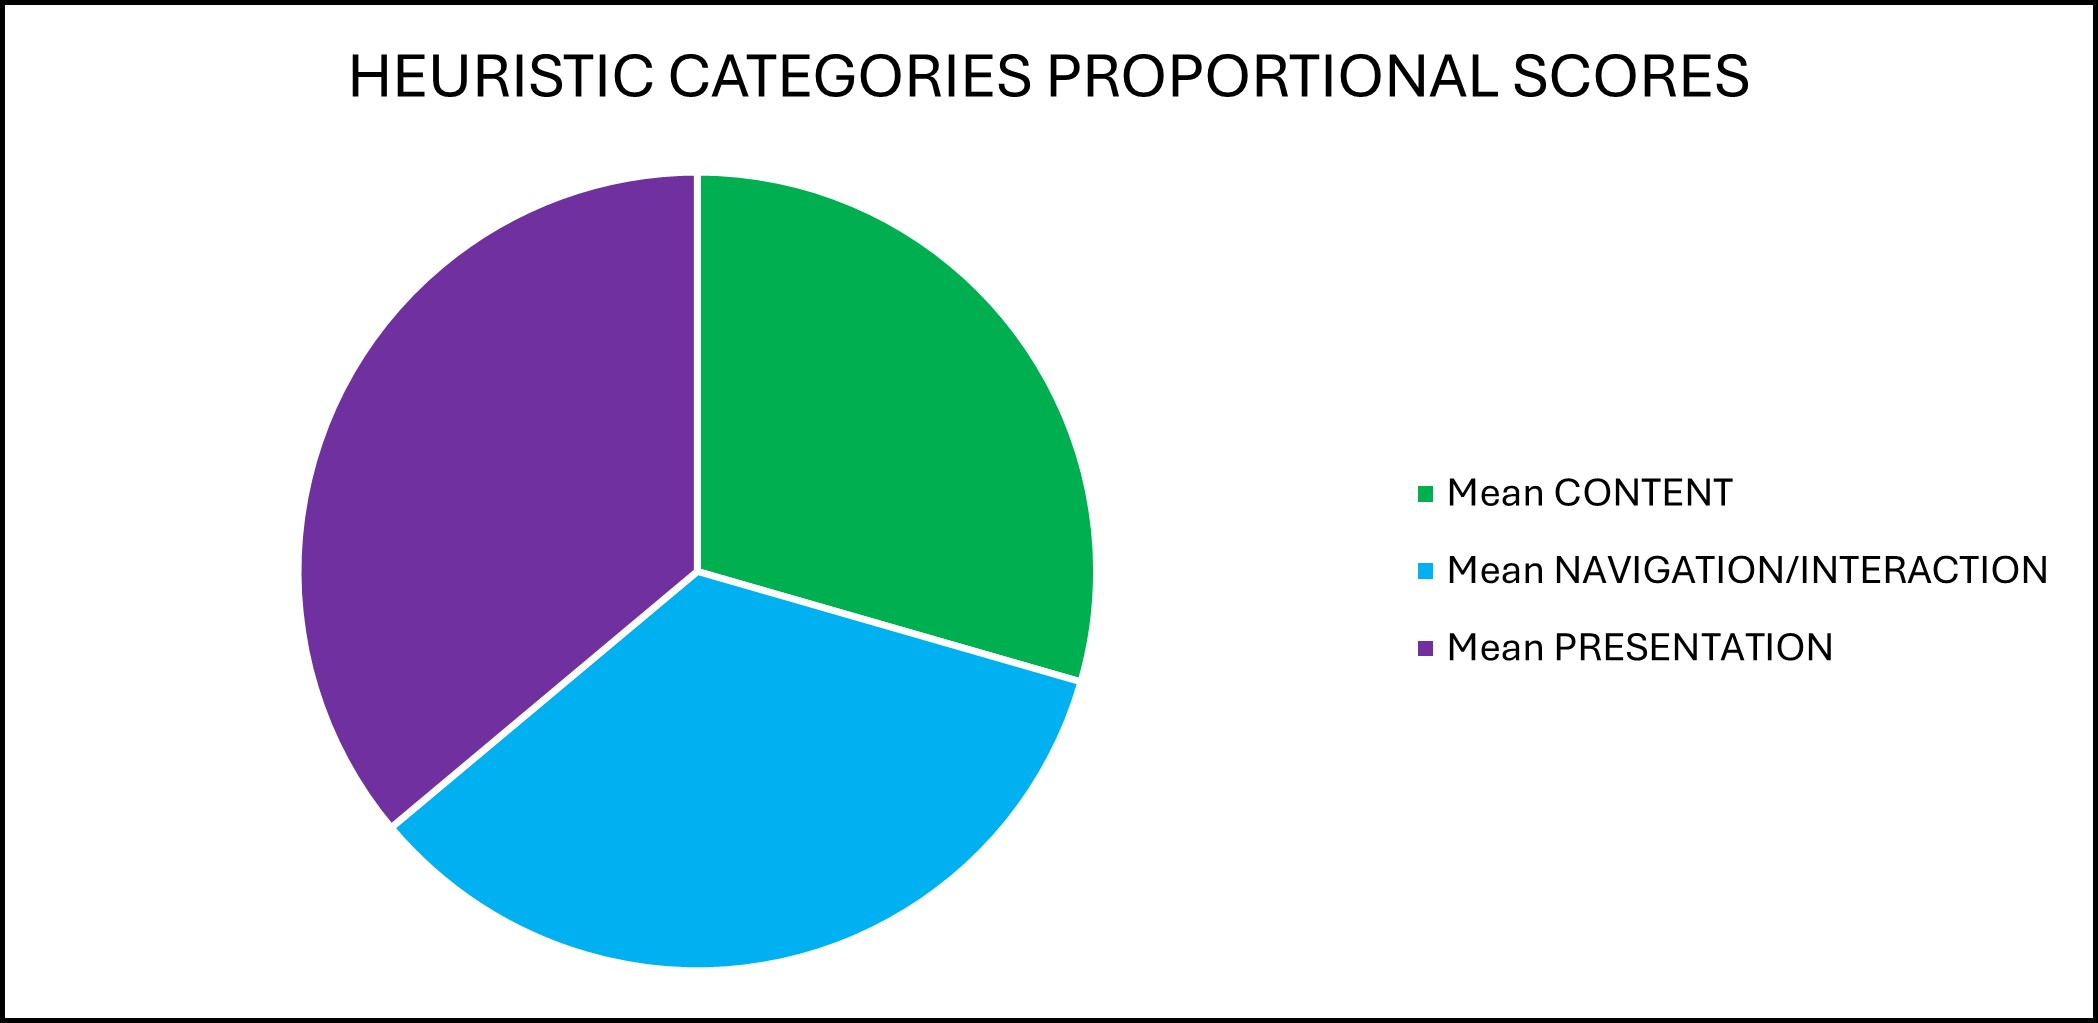
\includegraphics[width=\textwidth]{Visual_illustration_1.jpg}
	\caption{\textit{HEURISTIC CATEGORIES PROPORTIONAL SCORES.}}
	\label{fig:label1}
\end{figure}
\begin{figure}[h]
	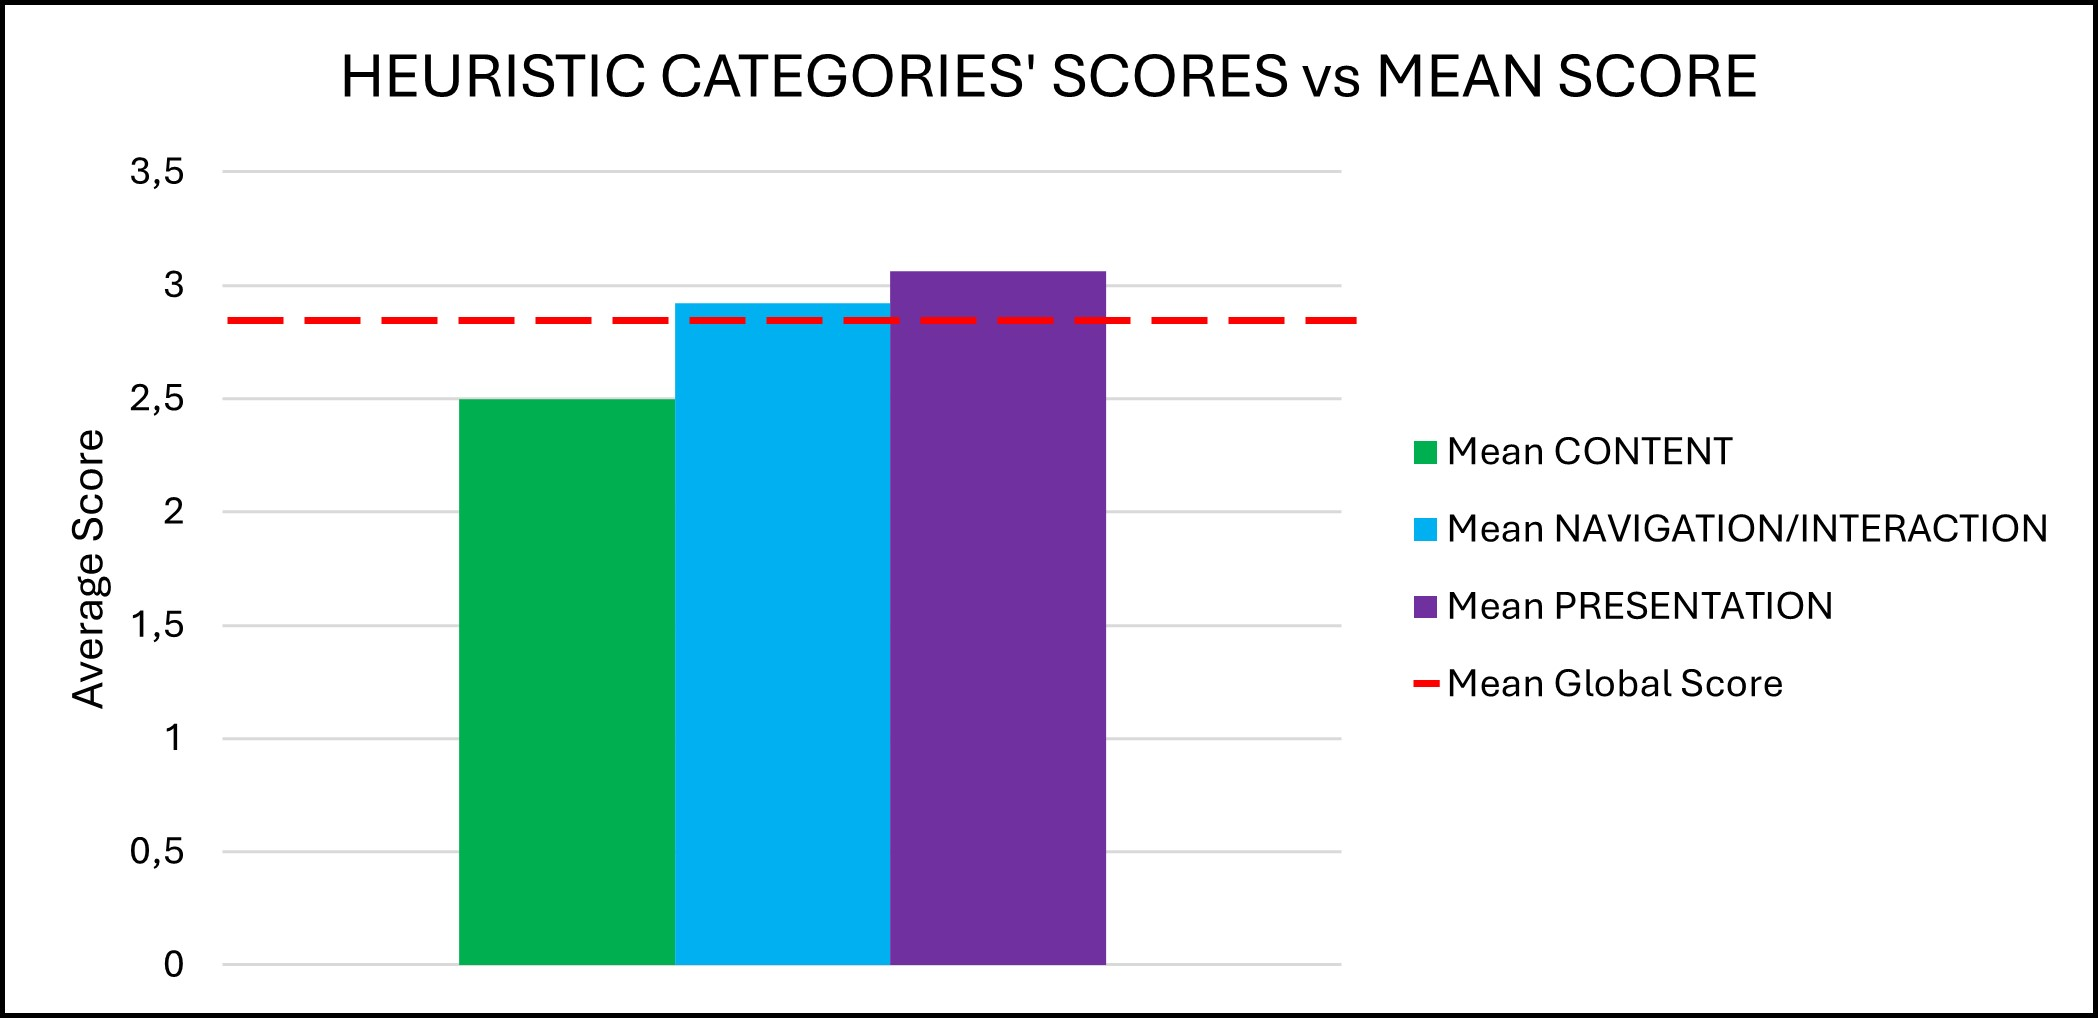
\includegraphics[width=\textwidth]{Visual_illustration_2.jpg}
	\caption{\textit{HEURISTIC CATEGORIES' SCORES vs MEAN SCORE.}}
	\label{fig:label2}
\end{figure}
\begin{figure}[h]
	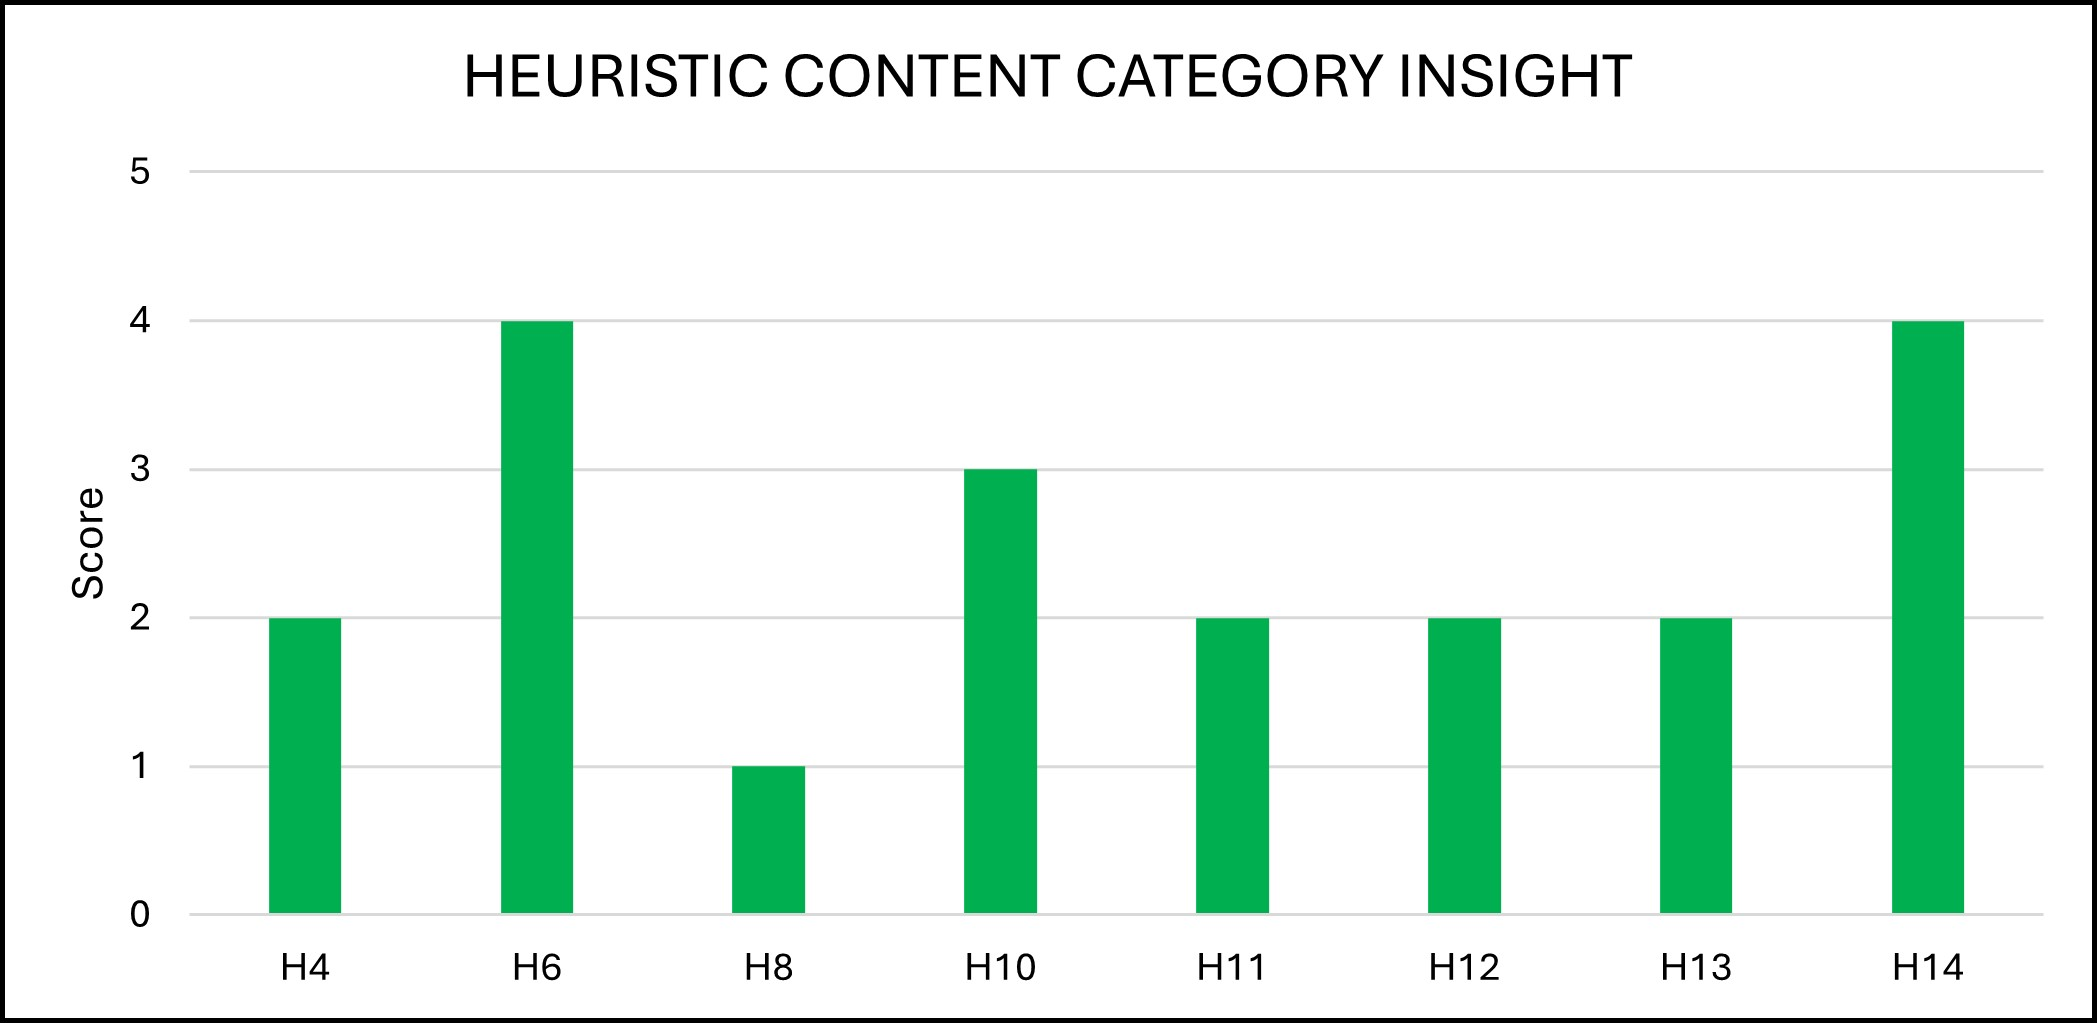
\includegraphics[width=\textwidth]{Visual_illustration_3.jpg}
	\caption{\textit{HEURISTIC CONTENT CATEGORY INSIGHT.}}
	\label{fig:label3}
\end{figure}
\begin{figure}[h]
	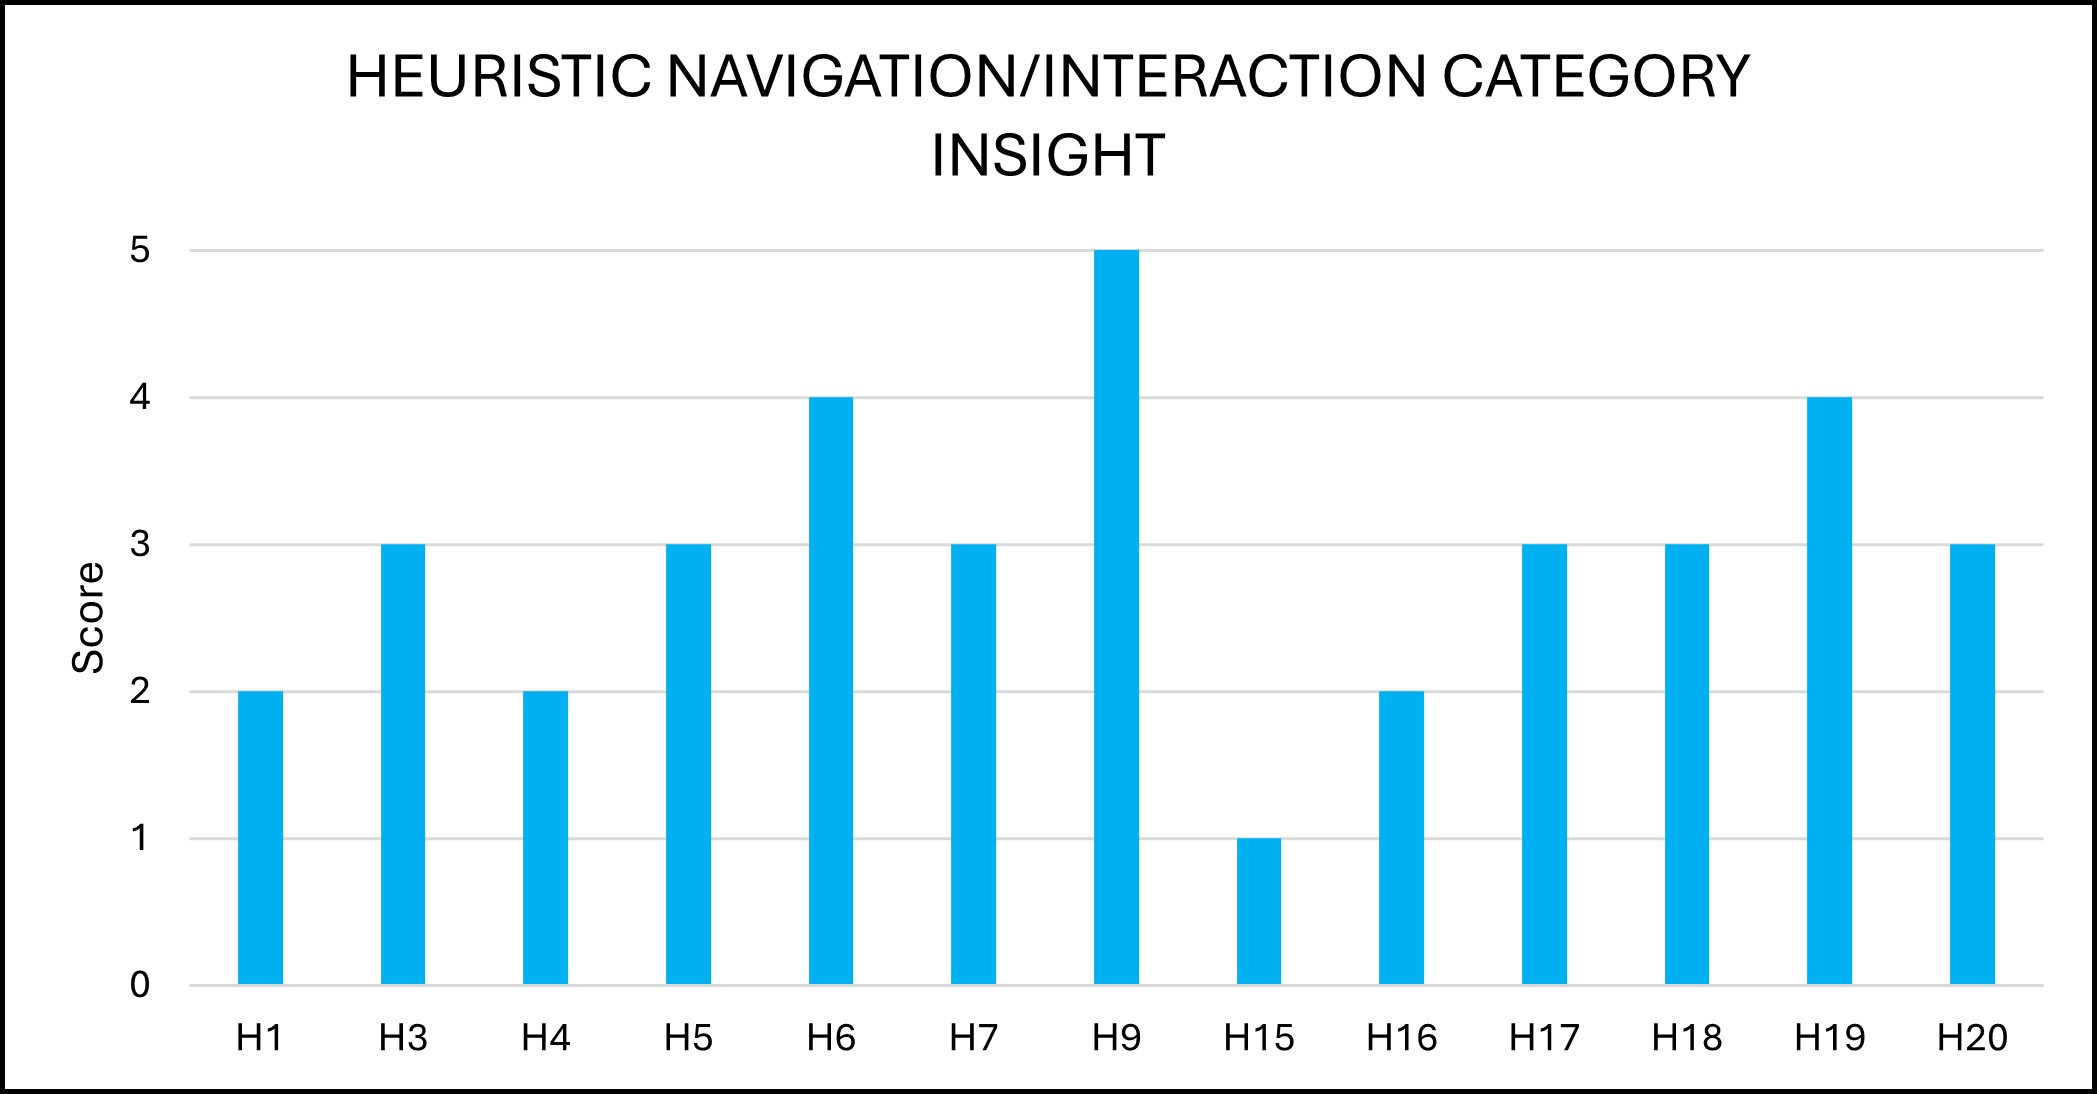
\includegraphics[width=\textwidth]{Visual_illustration_4.jpg}
	\caption{\textit{HEURISTIC NAVIGATION/INTERACTION CATEGORY INSIGHT.}}
	\label{fig:label4}
\end{figure}
\begin{figure}[h]
	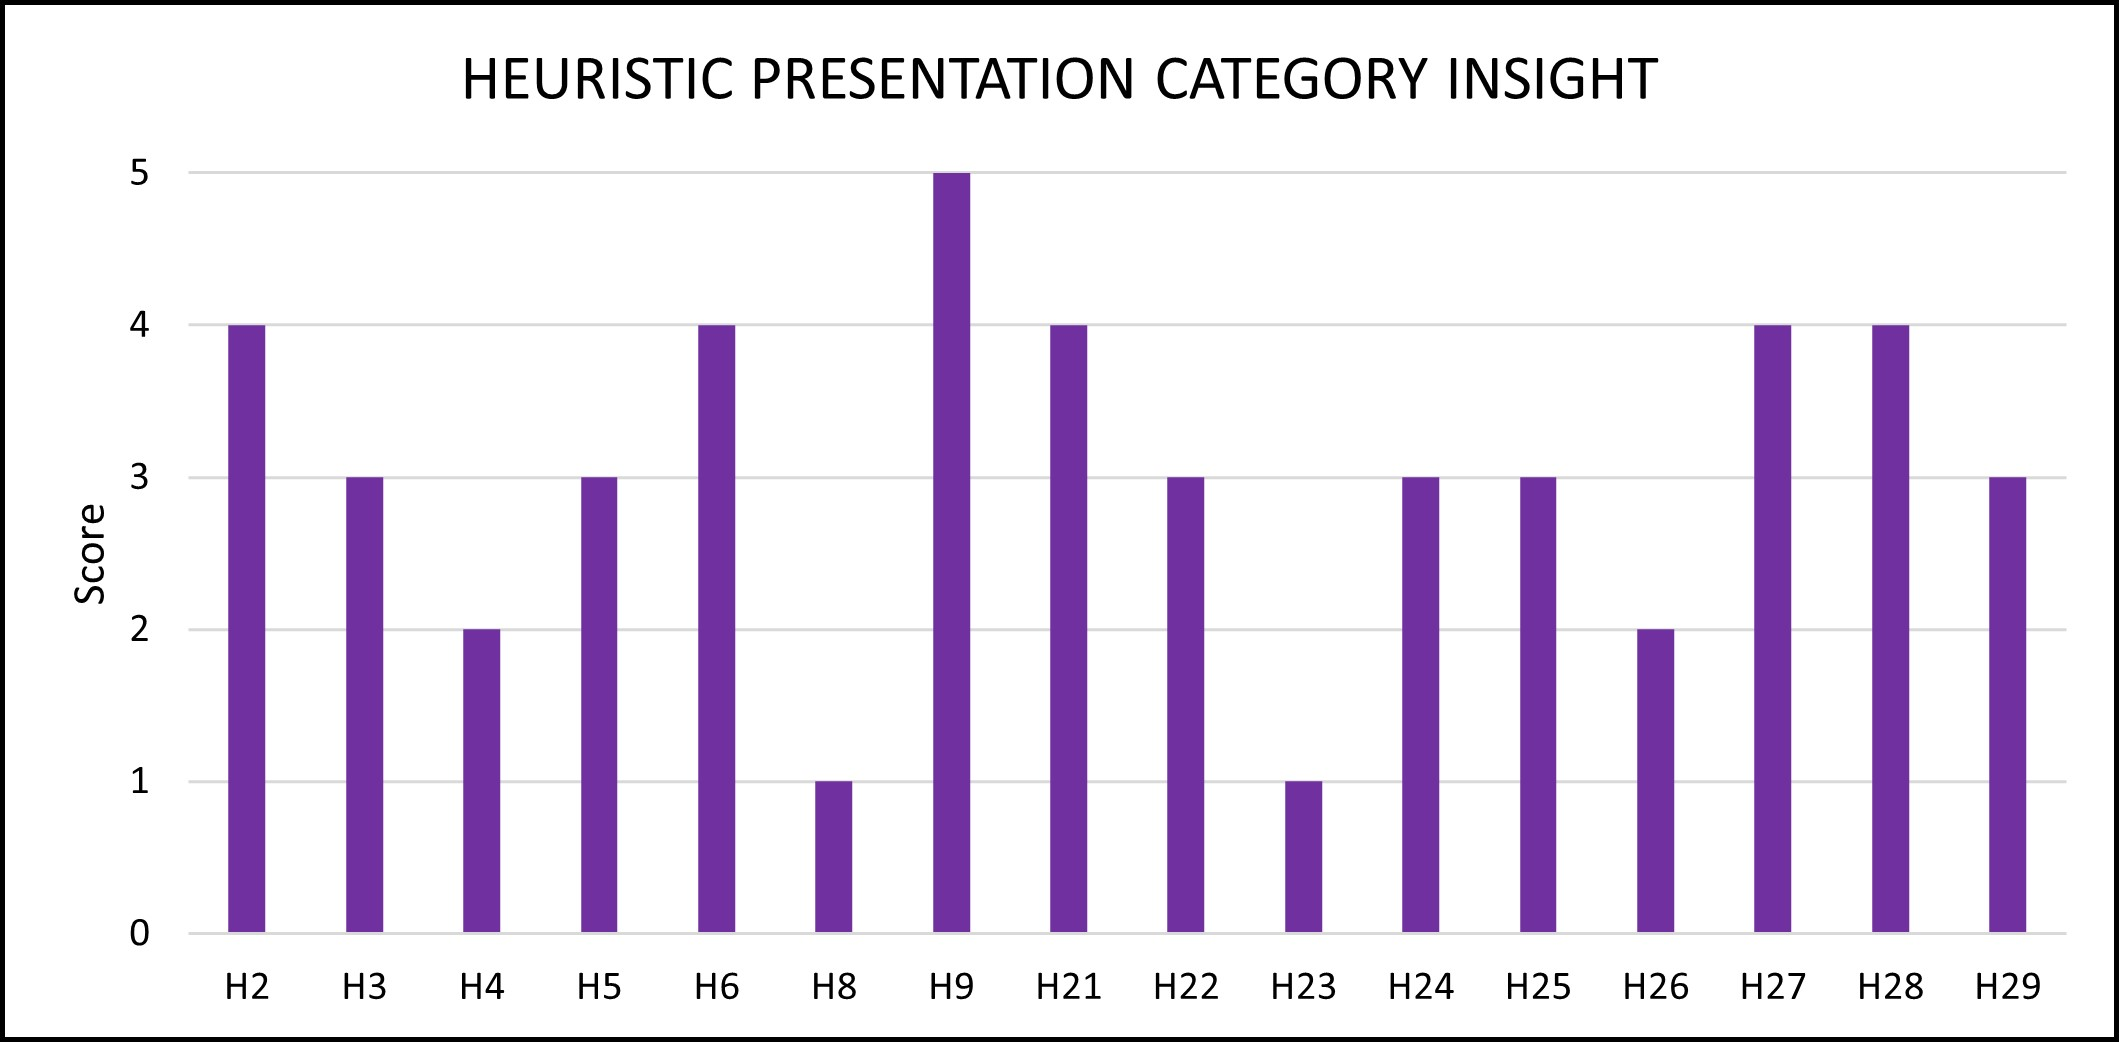
\includegraphics[width=\textwidth]{Visual_illustration_5.jpg}
	\caption{\textit{HEURISTIC NAVIGATION/INTERACTION CATEGORY INSIGHT.}}
	\label{fig:label5}
\end{figure}
